{
\begin{figure*}[th]
\begin{minipage}{\columnwidth}
\begin{center}
\centerline{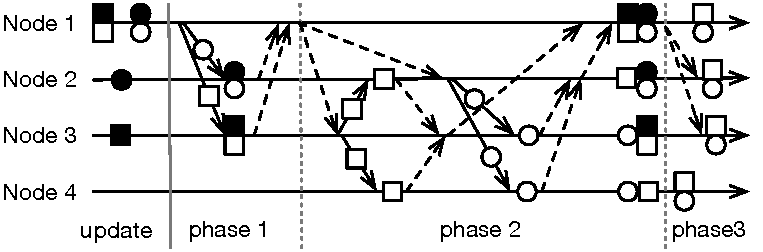
\includegraphics[width=\columnwidth]{Figures/commit.pdf}}
\vspace{-0.05in}
\mycaption{fig-mrmw}{\mrmw\ Commit Example.}
{
Solid arrows represent data communication.
Dashed arrows represent metadata communication.
Node 1 (\xn) commit data to \on{}s at Node 2 and 3 with replication degree four.
Black shapes represent old committed states before the update
and white shapes represent new states.
}
\end{center}
\end{minipage}
\begin{minipage}{\columnsep}
\end{minipage}
\begin{minipage}{\columnwidth}
\begin{center}
\centerline{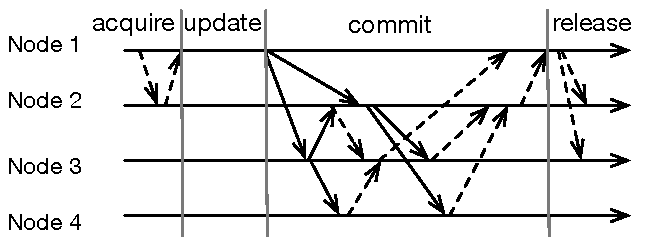
\includegraphics[width=0.42\textwidth]{Figures/mrsw.pdf}}
\vspace{-0.05in}
\mycaption{fig-mrsw}{\mrsw\ Example.}
{
Node 1 (\xn) first acquires write permission from Node 2 (\master)
before writing data.
It then commits the new data to \on{}s at Node 2 and 3 with replication degree four
and finally releases the write permission to \master.
}
\end{center}
\end{minipage}
\vspace{-0.3in}
\end{figure*}
}
